\section{Stakeholder Management}
\label{sec:stakeholders}
\lhead{\thesection \space Stakeholder Management}

Stakeholder Management includes the processes required to identify the people, groups and organizations that could affect or be affected by the project, to analyze stakeholder expectations and their impact on the project, and to develop appropriate strategies and tactics for effectively engaging stakeholders in a manner appropriate to the stakeholders interest and involvement in the project. Stakeholder Management helps to ensure that stakeholders are effectively involved in project decisions and execution throughout the life cycle of the project, to gain support for the project and anticipate resistance, conflict, or competing objectives among the project’s stakeholders.

\subsection{Identify Stakeholders}

In order to develop an effective plan for managing stakeholders, they first need to be clearly identified and assessed. Stakeholders will be identified by performing a stakeholder analysis in which potential stakeholders and relevant information (interests, involvement, inter dependencies, influence, and potential impact on project success) are gathered, documented and analyzed. 


\begin{table}[H]
\centering
\begin{tabular}{|c|c|}
\hline
\cellcolor{gray}Name & \cellcolor{gray}Description \\ \hline
Guido Bruzniak & Product owner \\ \hline
Marco Kull & Quality Manager \\ \hline
Sebastian Wilczek & Software Architect \\ \hline
Patrick Richter & Project Leader \\ \hline
Lucas Gehlen & Scrum Master \\ \hline
Thijs Dorssers & Docent \\ \hline
\end{tabular}
\caption{Stakeholders}
\end{table}

For this project six stakeholders were identified. To assist with stakeholder identification and analysis, the team has created and is completing a Stakeholder Analysis Register categorized by Stakeholder Group. The Stakeholder Analysis Register captures the following information
\newline
\newline
•	Group Name
\newline
•	Number of Stakeholders in the Group
\newline
•	Description of the Group
\newline
•	Level of Impact on the Project
\newline
•	Level the Group is Impacted by Project
\newline
•	Current Change Readiness State
\newline
•	Desired Change Readiness State
\newpage
A snapshot from the Stakeholder Analysis Register is provided below.
Please note: Impact is measured by High (H), Medium (M) or Low (L).  State of change readiness is assessed using the measures from \textit{Project Management Body of Knowledge} (PMBOK) 5th Edition  as follows: 

U - Unaware – this group has no information about the project
\newline
R – Resistant – aware of project and resistant to the changes and impacts the project may bring
\newline
N – Neutral – aware of the project and neither supportive nor resistant
\newline
S – Supportive – aware of the project and the potential changes and impacts and is supportive 
\newline
L – Leading – aware of the project and actively engaged to ensure the project’s success
\newline

\begin{table}[H]
\centering
\begin{tabular}{|c|c|c|c|c|c|c|}
\hline
\cellcolor{gray}\begin{tabular}{@{}c@{}}Group\\Name\end{tabular} & \cellcolor{gray}\# in Group & \cellcolor{gray}Description & \cellcolor{gray}\begin{tabular}{@{}c@{}}Impact on\\Project\end{tabular} & \cellcolor{gray}\begin{tabular}{@{}c@{}}Impacted by\\Project\end{tabular} & 
\cellcolor{gray}Current State & \cellcolor{gray}Desired State  \\ \hline

\begin{tabular}{@{}c@{}}Project\\Team\end{tabular} & 4 & \begin{tabular}{@{}c@{}}The project\\team\end{tabular} &
High & Low & L & L \\ \hline

\begin{tabular}{@{}c@{}}Product\\Owner\end{tabular} & 1 & \begin{tabular}{@{}c@{}}The product\\owner\end{tabular} &
High & High & L & L \\ \hline

Coach & 1 & \begin{tabular}{@{}c@{}}The coach\\of the \\ project team\end{tabular} &
Low & Low & S & S \\ \hline

\end{tabular}
\caption{Stakeholder Analysis Register}
\end{table}

\subsubsection{Power/Interest Classification}
As mentioned above, the Connected.Football SOFA project is assessing each group’s position, as well as their impact on the project and/or how they are impacted by the project.  One purpose of this activity is to help identify and categorize groups so that appropriate attention can be given to each group according to the level of engagement needed.  To help in this process, the project will use the PMBOK Power/Interest Grid to categorize each stakeholder group.  The Power/Interest Grid analyzes stakeholder groups in a visual manner to further establish stakeholders level of interest or concern and their ability to influence the project outcomes. 
\newline
An important outcome of the stakeholder identification and analysis work, including the Power/Interest Grid, is to identify the most influential and most impacted stakeholder groups so that a focused stakeholder management strategy and plan can be developed and executed.

\begin{figure}[H]
  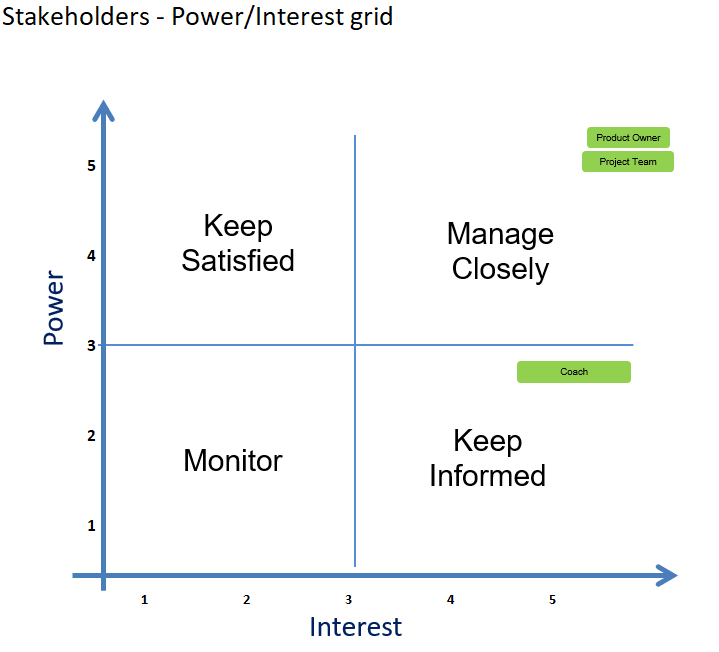
\includegraphics[width=\linewidth]{content/diagram/stakeholder/power_interest.png}
  \caption{Power/Interest Matrix}
\end{figure}

\subsubsection{Stakeholder Interviews}
In addition, optional qualitative interviews may be performed for the Stakeholder Groups identified as most influential or most impacted by the project to validate that their issues and concerns have been captured accurately.

\newpage

\subsection{Plan Stakeholder Management}
%Plan Stakeholder Management is the process of developing appropriate management strategies to effectively engage stakeholders throughout the lifecycle of the project, based on the analysis of their needs, interests and potential impact on project success. The key benefit of this process is that it provides a clear, actionable plan to interact with project stakeholders to support the project’s interests (PMBOK 5th Edition). 
%\newline
%\newline
Based upon the information gathered in the Stakeholder Analysis Register and the Communication Management, the Project Manager will be responsible for engaging stakeholders throughout the life cycle of the project. The level of engagement required for each stakeholder may vary over the course of the project. For example, during the beginning stages of the project, it might be necessary for the Project Manager to engage key stakeholders to be highly engaged.  Highly engaged key stakeholders in the early stages of the project are pivotal for project kickoff, achieving staff buy-in and clearing obstacles.  As the project progresses, the level of engagement will shift from key stakeholders to the broader project team and end-users.  

\subsubsection{Stakeholder Engagement}
To ensure the correct level of engagement is being achieved by each stakeholder, the Project Manager will analyze current levels of engagement by using the PMBOK Stakeholders Engagement Assessment Matrix.  As noted above in the Stakeholder Analysis Register, each stakeholder group shall be assessed in terms of their current and desired level of engagement.
 
 \begin{table}[H]
\centering
\begin{tabular}{|c|c|c|c|c|c|}
\hline
\cellcolor{gray}Stakeholder & \cellcolor{gray}Unaware & 
\cellcolor{gray}Resistant & \cellcolor{gray}Neutral & 
\cellcolor{gray}Supportive & \cellcolor{gray}Leading\\ \hline

Guido Bruzniak & / & / & / & / & C/D \\ \hline
Marco Kull & / & / & / & / & C/D   \\ \hline
Sebastian Wilczek & / & / & / & / & C/D   \\ \hline
Patrick Richter & / & / & / & / & C/D    \\ \hline
Lucas Gehlen & / & / & / & / & C/D   \\ \hline
Thijs Dorssers & / & / & / & C/D  & / \\ \hline

\end{tabular}
\caption{Stakeholder Engagement Assessment Matrix}

\end{table}

\subsection{Manage Stakeholder Engagement}

%Stakeholder Engagement Management is the process of communicating and working with stakeholders to meet their needs and expectations, and to address issues as they occur. Stakeholder Engagement Management is the process to systematically foster appropriate stakeholder engagement in project activities throughout the life of the project. The key benefit of this process is that it allows the Project Manager to increase support and minimize resistance from stakeholders, significantly increasing the chances to achieve project success (PMBOK 5th Edition).
%\newline
%\newline
To effectively manage stakeholder engagement, the Connected.Football SOFA Project will utilize the Communication Management part and strategies identified above to communicate project related information to key stakeholders in a proactive and timely manner.  Leveraging the information provided in the Communication Management (i.e., stakeholder groups, communication items, purpose, method of communication, and frequency), the project will have the ability to increase support and minimize stakeholder resistance throughout the life of the project.  Managing stakeholder engagement helps to increase the probability of project success by ensuring that stakeholders clearly understand the project goals, objectives, benefits, and risks. 
\newline
In line with the analysis above, the project team will also be actively listening and soliciting input and feedback to make sure communications are being received and understood, and also to capture important information to help make adjustments and to respond to problem areas.
\newline
Other project artifacts will factor into Stakeholder Management as well, including the list of Business Process Changes and the Change Control process, both of which consider the impact on stakeholders.  The project Issues Log is another tool to collect, document, and address concerns raised by stakeholders and stakeholder management risks that have materialized into issues that must be managed.

\subsection{Monitor Stakeholder Engagement}
%Monitor Stakeholder Engagement is the process of monitoring overall project stakeholder relationships and adjusting strategies and plans for engaging stakeholders.  Monitor Stakeholder Engagement involves collecting data, assessing the level of engagement and using insights from the data collection to adjust strategies and tactics for engaging effectively with stakeholders.
%\newline
%\newline
As mentioned in the Communication Management and the Risk Management, the Connected.Football SOFA Project will have mechanisms to receive ongoing direct feedback from key stakeholders. Individual stakeholders will be encouraged to participate and to voice questions and concerns, with the most serious issues and concerns that are raised addressed in a formal, rigorous process through the Issues and Risk logs.
\newline
\newline
As described in the Scope Management, the project will solicit broad participation in the collection and validation of requirements, which will uncover issues and concerns early on so they can be addressed.
Stakeholders are critical to the project’s success.  The project team has planned for and will work to involve, engage and listen to all key stakeholders throughout the project life cycle.

\subsubsection{Stakeholder Plan Updates}
Note that the Stakeholder Management Plan and associated documents are not static.  The stakeholders identified and their information documented in the Stakeholder Analysis Register will be reviewed at least monthly to ensure the plan is meeting project expectations and to make modifications if required.